% !TeX encoding = UTF-8 Unicode
% !TeX program = xelatex+makeindex+bibtex
% !TeX spellcheck = sk-SK
%
\documentclass[11pt,a4paper%,twoside
]{article}
\usepackage{fontspec}
\setmainfont[Numbers=Lining]{Linux Libertine O}
\newcommand{\noteDynamics}[2][1.3]{\raisebox{0.05ex}{\fontspec[Scale=#1]{Emmentaler-11}{#2}}}
\usepackage{polyglossia}
\setdefaultlanguage{slovak}
\setotherlanguage{english}
\setotherlanguage{french}
%\usepackage{tocloft}
%\setlength\cftparskip{-2pt}
%\setlength\cftbeforesecskip{0.5em}
%\setlength\cftaftertoctitleskip{2pt}
\usepackage{xcolor}
\usepackage{natbib}
\usepackage{hyperref}
\definecolor{printblue}{rgb}{0,0,0.8}
\definecolor{proofreadcolor}{rgb}{0.0157,0.5176,0.2666}
\definecolor{attentioncolor}{rgb}{0.8235,0.2666,0}
\hypersetup{bookmarksnumbered=true,
bookmarksopen=false,
pdfpagemode=UseNone,
hypertexnames=false,
colorlinks=true,
urlcolor=printblue,
filecolor=printblue,
linkcolor=printblue,
citecolor=printblue,
anchorcolor=printblue,
hypertexnames=false,  
pdftitle={Dodatok ku knihe Základy cvičenia na klavíri},
pdfauthor={Chuan C. Chang},
pdfsubject={Metódy a techniky cvičenia na klavíri},
pdfkeywords={klavír, piano, cvičenie, technika, ladenie klavíra},
unicode=true,
pdfstartview=FitH}
\usepackage[left=1in,top=1in,right=1in,bottom=1in%,bindingoffset=0.5in
]{geometry}
\makeatletter
\DeclareRobustCommand{\em}{\@nomath\em\if\expandafter\@car\f@series\@nil\normalfont\else\it\bfseries\fi}
\makeatother
\title{Dodatok ku knihe \emph{Základy cvičenia na klavíri}}
\author{Chuan C. Chang}
\date{pôvodný dokument z 25. augusta 2014,\\preklad z \today}
\begin{document}
\maketitle
%\begin{center}Translation \copyright\ \the\year\ Ladislav Rado%, \href{mailto:lr@rsw.sk}{lr@rsw.sk}
%\end{center}
Tento dodatok obsahuje materiál, ktorý bude zahrnutý v ďalšom vydaní knihy Základy cvičenia na klavíri, ak a keď bude napísaná. Ocením akékoľvek nápady/pripomienky, pretože táto stránka je stále vo výstavbe. Prosím, napíšte mi na \href{mailto:cc88m@aol.com?subject=Addendum\%20Comments}{e-mail} svoje pripomienky.
Návrat na \href{http://www.pianopractice.org/}{domovskú stránku} (Fundamentals of piano practice).

\tableofcontents

\section*{Errata}
\addcontentsline{toc}{section}{Errata}
%(poznámka prekladateľa: opravy sú už zahrnuté v preklade)

%str. 54: 3. odsek, prvé dve vety. "...mäkký pedál správne. Ak je pedál..." by malo byť
%“...  pravý pedál správne (účinok je zanedbateľne malý pre mäkký pedál). Ak sa pravý pedálu...”\smallskip\\
%str. 58: držať oktávu 35; 35 by malo byť 31\smallskip\\
%str. 88: veľkosť šmykové by mala byť naprostá veľkosť, 1. odsek.\smallskip\\
%str. 89: vyhlásenie v tom zmysle, že "palec by mal byť hraný ako akýkoľvek iný prst" nie je striktne
%správne, pretože palec hrá väčšinou rotáciou predlaktia, pozri odstavec 5 nižšie.\smallskip\\
%str. 96: (-1), by mala byť A (0), 3. odsek.\smallskip\\
%str. 125: namiesto “automatizácia” by mala byť “automatický”, v 3. odstavci.\smallskip\\
%str. 172: "rýchlosť zvuku v plodovej vode sa líši od toho v vzduchu s výsledným zmenou
%zdanlivý frekvencie "je zlé. Frekvencia sa nemení. Tak vystavovať deti k hudbe pred narodením
%môže im pomôcť rozvíjať hudobne, získať absolútnu sluch alebo rozvíjať koncept rytmu. Tam je teraz
%vedecké dôkazy, že mnoho detí z nosníc druhu komunikovať so svojimi rodičmi, zatiaľ čo ešte v
%vajcom, pred liahnutím.

\section*{Úvod}
\addcontentsline{toc}{section}{Úvod}
Tento dodatok je príkladom toho, čo mám na mysli pod tým, že “táto kniha nie je hotový produkt, je to len začiatok” (na zadnej obálke knihy). Budúcnosť klavírnej pedagogiky má neobmedzený potenciál a ako ďaleko to pokročí záleží len na našom úsilí a metódach, ktoré používame na štúdium toho, ako študovať. Pozri oddiel 7, o tom, čo sa rozumie pod “neobmedzeným potenciálom”. Táto kniha nie je jediným priekopníkom postupujúcich metód výučby klavíra; v súčasnosti existuje celý rad internetových serverov a učiteľov, ktorí aplikujú moderné metódy výuky klavíra s podobnými výsledkami (pozri knižné recenzie, dole), napriek tomu je táto kniha najobsiahlejšia v tejto dobe. Tento jav je dôsledkom rozvoja vzdelávania vo všeobecnosti, čo nám napovedá, že vyššie vzdelávanie mimo oblasť hudby bude stále viac  užitočné a potrebné pre budúcich klaviristov a najmä učiteľov klavíra.

Najdôležitejšia hudobná/biologická lekcia tejto knihy je, že hudba je mimoriadne užitočné zariadenie pre rozvoj ľudského mozgu (sekcia 1 nižšie), a že učitelia môžu ovládať tento vývoj. V minulosti hudobná pedagogika príliš často ignorovala túto možnosť (alebo o nej nevedela) a pripisovala pokrok študentov talentu. Niektoré podrobnosti o tom, ako cvičiť pre rýchlosť a ako učiť sú uvedené nižšie, oddiely 3, 4, 5 a 8.

Najdôležitejšie praktická lekcia tejto knihy je projektové riadenie (pozri bod 9): ako riadiť projekt od začiatku až do konca. Je to dôležité, pretože platia rovnaké princípy nielen pre učeniu na 
iné hudobné nástroje, ale aj pre každodenný život, školu, a prácu. Historické doklady ukazujú to, že Alexander Veľký použil podobné metódy na poraziť armády oveľa väčšej ako tej jeho.

Táto kniha obsahuje aj niekoľko nových objavov a metód výučby, ktoré nemožno nájsť v akejkoľvek inej literatúre; hlavné z nich sú uvedené v oddiele 10.

Oddiel 11 je môj pokus o vytvorenie teórie hudby postupom “zhora → nadol”. Môj názor je, že teórie majú zmysel, ak slúžia niekoľkým užitočným funkciám; teda užitočnosť tejto teórie je znázornená použitím Beethovenových sonát, naznačujúc to, že možno Beethoven používal niektoré podobné myšlienkové prúdy.

\section{Vytváranie géniov}
%Táto kniha sa zaoberá ľudským mozgom a ako ju použiť na výrobu hudby. Najväčší objav
%táto kniha je, že sme identifikovali postupy pre vytvorenie géniovia. Za týmto účelom, musíme definovať, čo génius je. Prodigy, talent a genius sú tu v podstate to isté. Môžeme rozlíšiť aspoň dva
%triedy géniov: Trieda I sa skladá z tých, ktorí získali toľko hudobné vedomosti a zručnosti, ktoré
%môžu vykonávať neuveriteľné hudobné výkony; Trieda II sa skladá z tých, s vrodenými hudobných myslí, taká, že s malým hudobným vzdelaním, môžu vykonávať tie isté neuveriteľné hudobné výkony. Diskusia o tom, či géniovia sa narodili, alebo vytvorené sú uvedené na stranách 16 a 202 knihy. Až do 1900s,
%Predpokladalo sa, že sa narodili (trieda II). Avšak, tam bol rastúci poznanie, že môžu
%byť vytvorená (16, P. Olsen). To je trochu analogické k teraz zdiskreditovanú presvedčenie, že niektorí sa rodia s absolútny sluch - nikto sa s tým narodil; každý musí sa to naučiť. V skutočnosti existuje dostatok dôkazov, že trieda I géniovia existujú, a že väčšina z tých, ktoré považujeme za géniovia sú typu I. triedy. Počet Géniovia II Trieda je extrémne malý a väčšina z nich má handicapy, ktoré bránia ich géniovia z plne vyvíja. \emph{Z toho možno vyvodiť, že väčšina slávnych géniov sú triedy I - boli vytvorené.} 
%
%Niet pochýb o tom, že vzhľadom skupinu rovnako pracovitých študentov s podobným zázemím, tam budú tí, ktorí budú vynikať a tí, ktorí sa nepodarí. Podobne, ak ste učiť absolútny sluch na skupinu mládež, niektorí sa naučia rýchlejšie ako ostatní. Je zrejmé, že ľudská populácia má rozdelenie mozgovej sily z veľmi zlá až veľmi dobré, a tak distribúciou tiež existuje pre hudobnosť. Tí, ktorí sa hudobný mozog nad určitý bod v tejto distribúcie sú označené ako géniovia. Využime Gaussian
%Distribúcie pre túto diskusiu, pretože toto rozdelenie zodpovedá prekvapivo veľký počet skutočných
%rozvody v reálnom svete a mala by byť dobrou reprezentáciu hudobníkov:
%
%\begin{figure}[!ht]
%\centering
%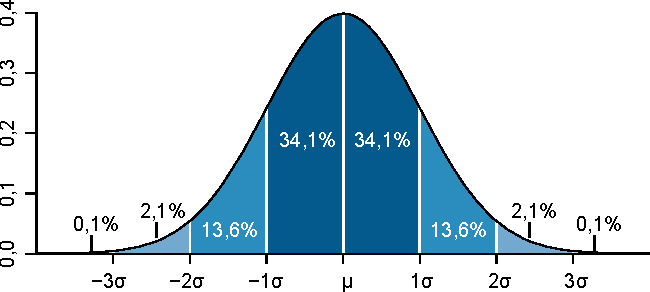
\includegraphics{Standard_deviation_diagram_(decimal_comma).pdf}
%\caption{Gaussovo rozdelenie}
%\label{fig:gauss-distribution}
%\end{figure}
%
%Horizontálna os predstavuje inteligenciu, alebo učenie rýchlosť, a na zvislej osi je podiel
%Študenti s touto inteligenciou. Centrum je označený písmenom "mu" a dôležité body sú označené
%o 1, 2 sigma sigma, atď. Plocha pod krivkou predstavuje počet študentov v rámci ktorej
%inteligencie rozsah. Väčšina študenti hudby spadajú do tmavej oblasti okolo polovice (68,2\%); rýchly
%študenti spadajú do svetlejších oblastí vpravo a učia pomaly, sú na ľavej strane. Dajme tomu, že tie, ktoré sme označiť ako hudobný géniovia tvoria 0,1\% populácie študentov, podľa označenia na krajnej pravici. Teraz, ak úžasný nový spôsob výučby boli zistené tak, že každý študent zlepšuje, celá krivka sa posunie vpravo, tak, že, napríklad, 2,1\% študentov vykonávať rovnako ako predchádzajúce 0,1\% Genius, as označené na distribúciu. Počet géniov sa zvýšil o faktor 20! Ohromujúca
%Dôsledkom je to, že neexistuje žiadny dôkaz, že dnes distribúciu nemožno tlačená tak, aby 50\% alebo viac populácia môže byť zvýšený na dnešnej úrovni, geniálny riadne vzdelanie a ďalšie prostriedky ešte byť objavil, pozri bod 6 vyššie (vedecká metóda).
%Vedomosti tak môže nahradiť surovou mozog moc. Ak chcete vidieť, že by sme brať priemernú 5. porovnávač dnes a časovo portov ho späť do Egypta pred 8000 rokmi a predpokladám, že sa zapísal všetko, čo vie o matematike. On by boli zaznamenané do histórie ako najväčšia matematický génius všetkých čias!
%Ak je táto kniha, a objavujúce sa moderné metódy výučby, sú rovnako revolučné ako posudkami
%ktoré obdržali naznačujú, tam bude oveľa viac géniovia v blízkej budúcnosti, než v súčasnej dobe existuje. Tento by sa mala vzťahovať nielen na klavírny techniky a vystúpenia, ale aj na skladanie hudby, originality, a vynaliezavosť. Lepšie metódy výučby, môže mať za následok mnoho ďalších Mozartom, Beethovens a Chopins na budúcnosť. Dobré metódy výučby môže vytvoriť géniovia!
%Aké sú niektoré z prvkov tohto geniálneho-vytváranie-konania? Pre podrobnosti, budete musieť čítať
%kniha, pretože množstvo vedomostí potreboval vykonať ho. My tu môžu zhrnúť niektoré
%prominentný body:
%
%(1) Je dôležité začať mladý, keď je mozog vyvíja a prispôsobuje sa na jeho prostredie.
%Historicky, slávny géniovia boli vytvorené svojimi rodičmi, ktorí boli už muzikanti, športové postavy,
%umelci, atď., a vedel, ako učiť svoje veľmi malé deti.
%
%(2) Metódy vyučovania / učenia sa musia dodržiavať správny proces riadenia projektu. Bez
%štruktúrovaný plán, bude väčšina projektov zlyhá. Pre hudobníkov, učenie na klavír, je jedným z najlepších štruktúrovaných plánov
%pre učenie riadenie projektu. Najdôležitejšie prvky v tomto pláne sú metódy praxe, ktoré
%zahŕňajú: Duševné Play, Absolute Pitch, memorization, klavírny techniky, Hudba Počúvanie a školenia,
%Znalosti (vysoká škola úroveň vzdelania), atď., Ako je uvedené v tejto knihe.
%
%(3), experimentovanie a sebestačnosť. Nemôžete spoliehať na nejaké hlavné učiteľov, aby sa vám do
%genius; musíte ovládať svoj vlastný rozvoj. Súčasťou tejto kontroly, však, je hľadať dobré
%Učitelia, ktoré môžu vopred svojich muzikálnosti, rovnako ako interakcie s vybranou skupinou hudobníkov, ktorí pochopiť "génia".
%
%Jedným zo spôsobov merania Genius je IQ (inteligenčný kvocient). K dispozícii sú tri úrovne, na ktorej je učenia klavír môže zvýšiť svoje IQ:
%
%(1) Máte vnútorný IQ - ako dobrý je váš mozog. To je najťažšie IQ zvýšiť, ale
%prevedenie hudobné výkony využije mozog takým spôsobom, že funguje lepšie, rovnako ako výkon vôle
%zväčšiť svaly a zvýšiť svoju silu. Jedným z cieľov cvičenia mentálne hra je
%zvýšenie mentálnej odolnosť a cvičiť mozog má fungovať po celú dobu bez nutnosti doby odpočinku a
%nečinnosť. Tým sa zvýši prietok krvi do mozgu a zvýšenie prekrvenia, zväčšením krv
%nádoby a robiť je pružnejšia, či dokonca zvýšenie množstva krvi v tele.
%
%(2) Váš efektívne IQ - ako dobre ste použiť silu mozgu, ktorý máte. Osoba, ktorá užíva
%Mozog efektívnejšie objavia múdrejší ako jeden s rovnakým mozgu, ktoré nevie, ako ju používať.
%Tento rozdiel môže byť nepochybne jasné, pre klavír, pretože klaviristi môže robiť veci na klavír
%že nie-klaviristi si absolútne nie. Tak to je ľahké pre klaviristu k zvýšeniu ich efektívne IQ na oveľa vyššej úrovniach, než ich vnútorné IQ. V skutočnosti, väčšina z tejto knihy je o metódach pre zvýšenie efektívneho IQ: metódy efektívnej praxe, ako je použitie paralelných sád rýchlo zrýchliť hru sú veľmi efektívne.
%
%(3) vnímaná IQ - ako iní ohodnotia svoje IQ. Mozarta, Beethovena, atď., Majú jedny z najvyšších
%vnímanej IQ. Jedinečnou vlastnosťou vnímanej IQ je, že môže byť zvýšený až dokonca aj nad efektívne IQ.
%
%V istom zmysle, že vnútorné a účinné IQ sú skutočné - by ste mali byť schopní navrhnúť metódy na meranie je. Vnímaná IQ je čisto "v očiach pozorovateľa"; to môže byť zvýšená na akejkoľvek úrovni použitím metód alebo triky, rovnako ako kúzelníci tomu, vykonať "zázraky". Prekvapivé je, že všetky hudobníkov to bežne, nech to robia vedome, alebo nie. V istom zmysle, hudobníci sú kúzelníci s ich vlastnými set trikov. Použitie hudby ako algoritmus do pamäte 5 hodín repertoáru je taký trik. Mozart použitý mentálna hra čítať vety pospiatky. Kombinácia duševné hru a Absolute Pitch je iný.
%Každý pianista mali byť vedomí týchto rôznych IQ a kultivovať ich - to je najrýchlejší spôsob, ako
%zvýšiť je tak vysoko, ako je to možné. Výsledkom je to, čo každý nazýva génius. Tu je čiastočný zoznam toho, prečo hudobníci majú tendenciu byť múdrejší ako ostatní: (1) učenie hudba je predovšetkým o zlepšenie mozog viac ako prsty. (2), hudobníci sa musí naučiť naspamäť. (3) hudobníci učí riadenie projektu a stať kvalifikáciou na plnenie úloh. (4), hudobník mozog musí vedieť, ako zaobchádzať s vysokou rýchlosťou (str 36). (5) prehrávanie hudby, hudobníci sú neustále hovorí s niektorými z najväčších géniov, ktorý kedy žil, a Tieto rozhovory utrieť na hudobník, ako je geniálny trikov a učenie triky. (6) hudobníci viac úspech mladší začnú, pretože ich mozgy začať ich výcvik skôr, keď mozgy sú pružnejšie, dlho predtým, než non-hudobníci sú vystavení tak komplexných konceptov a dlho pred rodičmi môže dodať takýto materiál. (7), hudba zahŕňa matematické, atď., Komplexné mozgu reakcie na (hlavne audio) vstupy (harmónie, akordu, melodické linky, atď.), ktoré pomáhajú rozvíjať silu mozgu. (8) produkujúce hudba vyžaduje neustálu, nepretržité spojenie, ktoré zvyšuje prietok krvi do mozgu a zvyšuje mozog výdrž. (9) hudobníci musia cítiť skvele minute rozdiely vo ihrisku, hlasitosť, načasovanie, atď, na zvuky a ovládať prstami a telo k ich vybavenie; tieto zvýšenej citlivosti vyžadujú viac rozvinutých mozgy. (10) hudba je jazyk, a učiť žiadny nový jazyk, vám dáva pridanú výhody učenie nových logické / koncepty a spôsoby komunikácie. Každý nový jazyk vám dáva nové možnosti, ktoré iné jazyky nemali; hudba nie je výnimkou, a je najúčinnejší, pretože sa jedná o univerzálnej jazykom. Atď.
%
\section{Mozartov vzorec}
%(viď stranu 206)
%
%Som lokalizoval profesor hudby, ktorý prednášal na vzorci Mozarta v decembri roku 1977 v Bell
%Laboratória pre výskum Kolokvium, v Murray Hill, NJ, ktoré je uvedené na P. 206 Je profesorom Robert
%Levin z Harvardu, ktorý hovoril o "Odtlačky prstov Mozartových: Štatistická analýza jeho koncertov"
%pokiaľ ide o "osobitné a sofistikovaný hierarchiu hudobných motívov, ktorá je základom Mozartov koncert
%forma "(Levin). Musím poďakovať Brian Kernighan (spoluautor "Programovací jazyk C"), pre
%umiestnenie záznamy k tejto prednáške, ktorá bola doteraz uložená v jeho počítači po viac ako 30 rokov. Po
%niekoľko e-mailové výmeny s Prof. Levin, som dorazil na nasledujúci opis udalostí, ktoré viedli k
%moja analýza Mozartova kompozičného mikroštruktúry diskutoval na P. 206; Pre podrobnejšiu analýzu
%Mozartova Sonáta op. 11 (K300), pozri Scoggin, P. 224.
%Prof. Levin neprerokovala mikroštruktúru Mozartových skladieb, ktoré som diskutovať v mojej knihe
%ale namiesto toho prednášal na hierarchiu hudobných motívov, ktoré boli natoľko špecifické, aby boli potenciálne užitočné pre
%overovanie Mozartových skladieb. Na jednej strane som bol sklamaný s prednáškou kvôli môjmu
%neznalosť hudobných motívov; Dúfal som, že počul, že tam bolo zrozumiteľnejšie muzikál
%štruktúra. Na druhej strane, Prof. Levin prebudila moje povedomie o štruktúre v hudbe. Som
%crystallographer, ktorý sa zaoberá atómovej štruktúry hmoty, takže to ma priviedlo k vedomia skúmať
%Mozartova hudba hľadať akúkoľvek štruktúru dosť jednoduché pre mňa poznať.
%Ako crystallographer, som zvyknutý náročné opakujúce mikroštruktúru záležitosti, ktorá
%určenie vlastností jednotlivých materiálov. Ak budete mať len jeden atóm, uhlík, môžete zmeniť atómový
%mikroštruktúra a dostať niečo z pevných, brilantné diamantov mazacie grafit ľahké golf
%klub hriadeľa a dokonca buckyballs s úžasnými vlastnosťami a použitie. Nebolo teda prekvapením, že
%opakujúce sa štruktúra Mozartovej hudby, vyskočil na mňa, hneď som si ju prezeral zo štrukturálneho hľadiska
%výhľad. Pre tých, ktorí nie sú zvyknutí na rokovania s mikroštruktúry, tento opakujúce sa štruktúra v hudbe nie je
%ľahko rozoznateľné, pretože to vyzerá, že má žiadny zrejmý význam pre melodickú progresiu. Mám
%testované toto uznanie so svojimi hudobnými kolegami a trvalo to väčšina z nich za to uvedomujú
%štruktúra ako súčasť hudby. Tento nedostatok uznania historicky zabránila plnenie tohto
%5
%mikroštruktúra, pretože pre hudobníkov, sa zdá, tak triviálne jednoduché, že to nezaslúži pozornosť. Jeden z
%Najlepším príkladom je pomalý pohyb Mozartovho klavírneho koncertu nie 21, ktorý je všeobecne
%považované za jednorazové, pretože neuveriteľné emocionálne obsah skryje opakovaní.
%Opakovanie, samozrejme, je kľúčom k väčšine hudbu. Taktu riadi celý kus, takže
%rytmus je 100\% opakujú. V rapovej hudbe, ako rytmus a melódie sú opakujúce sa, prevažne s textami
%mení. Mozartova hudba používa väčšinou jediný opakovania (2 ks v rade). Bach využíva opakovanie
%rozsiahlo, ale nie je obmedzený hlavne na jeden typ, ako je Mozart. V vynálezy, Bach používa 2
%opakovanie najčastejšie (3 ks v rade - pozri Invention \# 8). Opakovanie na väčšom meradle sú tiež
%dôležité, ako Ruth Slenczynska napísal: "prehrávať všetky repríz označené skladateľa" (Slenczynska - P. 49) -
%Pokyny zo skúsený pianista, pretože opakovanie je tam vyvolávať špecifickú reakciu
%publikum. Je jasné, že hudobníci musia vyvinúť hlboké porozumenie opakovanie a ako ich používať.
%Tieto typy opakujúcich sa štruktúr sú dobre známe medzi skladateľa, a články o hudbe
%Analýza a zloženie začínajú diskutovať o nich podrobnejšie (Brandt). Dokonca aj ihriská a sady
%symetria podobné tým diskutované na P. 209 (v Beethoven a teórie grup), sa objavili v
%literatúra (Bernard, Solomon).
\subsection*{Referencie}

\addcontentsline{toc}{subsection}{Referencie}

\section{Zapamätávanie si (ako na to, význam spánku)}
%Preberali sme metódy zapamätávania v sekcii III.6 a videli sme, že existuje najmenej päť typov pamäti: ručná pamäť, fotografická pamäť, hudobná pamäť, klávesová pamäť a teoretická pamäť. Prirodzená otázka, ktorá vyvstáva, je, “ktorú je najlepšie sa naučiť?"
%
%Odpoveď je “\emph{VŠETKY z nich!}”. Nebola by to strata času, ktorý by mohol byť lepšie využité na cvičenie vášho repertoáru? Poďme sa pozrieť, prečo sa \textit{potrebujeme} naučiť ich všetky.
%
%(1) Pamäť je asociatívna; Preto, aby ste sa skutočne naučili kompozíciu naspamäť, použitie všetkých metód pamätania si je potrebné pre maximalizovanie asociáci. To znamená, ako hudobníci, sa musíme pýtať sami seba, či chceme dokonalú pamäť alebo budeme spokojný len s čiastočným zapamätaním? Chcem byť skutočný profesionálny koncertný klavirista, alebo budem spokojný s tým, že budem amatérskym klaviristom?
%
%(2) Pre profesionálneho klaviristu, má každá metóda zapamätania si svoje konkrétne použitie. \textbf{Ručná pamäť} robí to skladbu jednoduchšie hrateľnou. Bez nej, mozog bude musieť poslať všetky inštrukcie na každý sval v celom Telo hrať aj jednoduché poznámky - bez ruky pamäti, mozog by bol úplne vyčerpaný v čase, budete hrať jednu stránku hudby. Je potreba fotografické pamäte pre vytváranie a testovanie svoju pamäť od klavíra. Jedná sa o spojenie medzi hudbou, ktorú hráte a pôvodné poznámky, z ktorého ste naučili hudbu. Obsahuje pôvodnú pokyny od skladateľa na umelcov. Je základným súčasť duševnej Play. Hudba pamäť je súčasťou základného algoritmu, ktorý nám umožňuje uložiť do pamäte Takmer nekonečné repertoár. To je dôvod, prečo sme sa dozvedeli na klavír! Nikto vykonáva bez hudby pamäte. Klávesnica pamäť je najužitočnejšia, keď sa učíte nový kus. Z tohto dôvodu, je to prvý pamäť metóda, ktorú vedome praxi. Teoretický pamäť je použitý pre analýzu zloženia a pochopenie toho, prečo niektoré poznámky sú tam, a pre automatické zapamätanie veľké kusy z Zloženie bez použitia fotografického alebo klávesnice pamäte. Všetky z pamäťových metódy môžu byť, a by mal byť použitý pre duševné hry. To sú len hlavné použitie; existuje mnoho ďalších. Prišli sme do Zistenie, že každá metóda pamäti spoločnosti s rôznymi vlastnosťami prostriedku, tak, že ak máme úplne zapamätať, je potrebné všetky pamäti metód.
%
%(3) V skutočnosti, je to strata času, nie sa naučiť ich všetky, pretože ak sa naučíte jeden z nich dobre, máte už naučili veľkej časti väčšina ostatných a môže naučiť sa komplexnejšie v krátkej dobe. Navyše, získate všetky výhody súvisiace s touto malé investície času. Ak nechcete dozvedieť všetko o im, ste skutočne zahodili tie isté zdroje, ktoré odlišujú génius z amatéra. Tieto body (1) - (3) vedie prirodzene k otázke, čo je najlepší postup pre učenie všetky z nich?
%
%V praxi sme automaticky učiť ručné pamäti, takže nemusíme cvičiť vedome.
%Ale musíme vedieť, čo to je, a podporiť jeho rast. Tiež sme videli, že klávesnica pamäť je prvá
%pamäť k praxi, pretože to je najužitočnejšia, keď najprv učí nový kus. Vzhľadom k tomu použiť hudbu konštatuje sa učiť zloženie, fotografická pamäť sa môže vykonávať v tomto okamihu a potom neskôr, v priebehu mentálne prehrávanie. Hudba pamäť je tiež automatické, najmä ak cvičíte hudobne. Teoretická pamäť je jediná, ktorá sa líši od osoby k osobe, pretože závisí na tom, ako veľmi teória viete. Miera, do akej je možné aplikovať teoretické pamäť závisí na vašej teórie vzdelanie. Avšak, dokonca aj bez pokročilých teórie vzdelania, každý môže urobiť štrukturálnej analýzy hudby, ktorý môže slúžiť ako teoretická pamäť.
%
%Prekvapenie! Došli sme k poznaniu, že učí všetky pamäti metód nasleduje prirodzene z procesu zapamätanie kompozíciu. To je jeden z dôvodov, prečo vykonávajúci priechod znovu a znovu nemusí byť nudné, pretože tam je toľko na práci.
%
%Správne spať v noci na deň zapamätanie akcie je zrejme dôležité pre trvalý pamäť; tam je veľa správ o tom teraz - stačí hľadať "pamäti, spánku" na internete. Ako skôr popísané (P. 108), to trvá asi 5 minút, pre mozog previesť krátkodobú pamäť až dlhodobom horizonte pamäť. Avšak, je tu ďalší "konsolidácia pamäť" proces, ktorý prebieha počas spánku, čo dáva zmysel, pretože sa vyskytujú rastové procesy, počas spánku (P. 42), a budovanie trvalej pamäti pravdepodobne zahŕňa niektoré druhy rastových procesov v mozgu. Tak pamäť má zložku PPI (Post Prax Improvement), rovnako ako vývoja techniky, takže môžeme využiť našej znalosti
%PPI (str 41) na zlepšenie pamäti. Kvalita spánku je dôležité najmä pre pamäte PPI.

\section{Metódy cvičenia  (rýchlosť, dotyk, farba)}

\subsection{Dôležitosť PS cvičenia č. 1}

\subsection{Získavanie techniky a rýchlosti ​​rýchlo}

\subsubsection{Rutinné cvičenie, spánok, pomalé hranie, dotyk, farba, tiché prsty, Chopinova Fantaisie Impromptu, výška stoličky}

\subsubsection{Cvičenie Staccato}

\subsection{Rýchle oktávy, malé ruky}

\subsection{Rutiny pre prípravu na vystúpenie: (prečo cvičenie v deň vystúpenia nefunguje)}

\subsection{Mýtus o vyučovacích metódach Frantza Liszta}

\subsection{Teória o získavaní techniky: vedomosti, experimentovanie a talent}

\subsection{Záhada “rozohrania sa”}

\section{Hranie s palcom}

\subsection{Rotácia predlaktia}

\subsection{Slabý/silný palec}

\subsection{Kľúčová pozícia pre hranie legato “palec cez”}

\section{Budúcnosť klavíra: digitálna revolúcia}

\section{Definovanie vedy a vedeckej metódy}

\section{Ako učiť na klavíri}

\subsection{Prvá lekcie}

\subsection{Následné lekcie}

\section{Riadenie projektu}
\ 

\subsection{Základné pravidlá}

\subsection{Príklad: Učenie sa absolútneho sluchu}

\subsection{Príklad: Starostlivosť o trávnik: Trávnik bez buriny}

\section{Nové metódy, vysvetlenia, a objavy tejto knihy}

\section{Teória hudby: s ilustráciami použitím Beethovenových sonát}

\subsection{Čo je to hudba?}

\subsection{Komunikačné médiá v hudbe: načasovanie, hlasitosť, výška tónu a logika}

\subsection{Jazyky hudby: rytmus, harmónia a melódia}

\subsection{Použitie hudobnej teórie na interpretovanie Beethovenových sonát: 1. vety z Moonlight, Pathétique, Appassionata}

\section{Nevýhody učenia sa na klavíri}

%%%%%%%%%%%%%%%%%%%%%% TODO %%%%%%%%%%%%%%%%%%%%%%%%%%%%%%%
\section*{Recenzie kníh}
\addcontentsline{toc}{section}{Recenzie kníh}
Recenzia knihy (\href{http://www.pianopractice.org/recommendedbooks.html}{kliknite tu} pre odkazy na Amazon Books)\\
\textbf{Bailie, Eleanor}, “Chopin: The Pianist's Repertoire, A Graded Practical Guide”, Kahn \& Averill, Londýn, 1998, 573P., Index osôb uvedených v knihe, bibliografia, index Chopin funguje. Napodiv nie je nič v knihe (alebo kdekoľvek inde) o Eleanor Bailie samotnej. \textbf{Odporúčaná}

Monumentálne kompendium (573 strán!) Prakticky všetkých dostupných informácií o Chopinových prácach, od histórie po technické detaily a interpretáciu.

Začína krátkymi posúdeniami všeobecných technických otázok (najmä to ako sa vzťahujú na Chopina), ale nie je to organizovaná učebnica pre učenie sa hrať na klavír. Príklady: Hrajte Bacha pre prípravu na vystúpenia, Chopinova hudba vychádza z Mozarta. Pianissimo je dôležitejšie ako \noteDynamics{ff}. Význam prísneho rytmu, a to najmä v ĽR. Chopinov prstoklad a pedálovanie, a to najmä ľavý pedál. Je tam sekcia s názvom “Chopinova výučba” ale obsahuje málo látky; namiesto toho sa odkazuje na (str. 23-64) zhrnutia v Eigeldingerovi.

Hlavná časť knihy je ~500 strán pripomienok na každej skladbe. Skryté vnútri týchto pripomienok sú početné rady, ako cvičiť, čo je samozrejme cenné pre každého, kto sa snaží naučiť tieto skladby; okrem toho, kompendium všetkých týchto rád by vyprodukovalo jednu z najlepších učebníc správnych metód cvičenia na klavíri. Preto táto kniha je pre klaviristov oveľa užitočnejšia než Eigeldinger.
\medskip\\
\textbf{Cook, Charles}, “Playing the Piano for Pleasure, Klasický sprievodca zlepšovania zručností prostredníctvom cviČenia a disciplíny”, Skyhorse Publishing, 2011, 187 P., žiadny index, má zoznam “konzultovaných kníh”. \textbf{Neodporúča sa}

Skromný Obsah a nedostatok indexu robí takmer nemožné nájsť žiadnu špecifickú tému v tejto knihe; naznačuje sa tým, aby ste si robili poznámky (s číslami stránok) prvýkrát, ako budete čítať knihu. Obsahuje niektoré dobré rady so zmesou s niektorými teraz zdiskreditovanými konceptami. Prečítajte si moju knihu pren touto, aby ste vedeli rozlíšiť medzi užitočnými a pochybnými radami. Jedná sa o aktualizované vydanie z roku 1960, a niektoré novších nápady vyvracajú staré nesprávne presvedčenia. Hlavne pre dospelých, vrátane začiatočníkov.

Napísaný z pohľadu amatérov, definovaných ako neprofesionálnych klaviristov, ktorí nemajú bežne musieť, ktorí nemusia vystupovať na požiadanie. To znižuje nároky na čas cvičenia a technické zručnosti a uľahčuje to aby bolo hranie na klavíri pre potešenie - preto ten nadpis. Avšak, za účelom udržania určitého typu repertoáru navrhuje (čo je rozhodujúce pre úspech) to, že amatérsky musí cvičiť hodinu každý deň. Toto je pochopiteľné; v porovnaní s ruku, ktorá nehrala týždeň je dobre podmienená ruka (tá istá osoba cvičila každý deň) bude vykonávať zázraky (toto je môj postreh - tento autor to výslovne neuvádza).

Napísané (hudobným) reportérom pre The New Yorker, s vážnym záujmom o klavír ako hobby, ktorý robil rozhovory s Horowitzom, Hofmanom, Schnabelom, Arrau, Rosenthalom, Brailowským, atď. Skúmal metódy učenia hry na klavíri s nahliadnutím do spisov slávnych klaviristov. Výborným príklad toho, ako vážny, usilovný klavirista/reportér môže mať mozog vymývaný rozhovormi slávnych osobností, ktorý ho kŕmia samoúčelnými vyhláseniami, ktoré z nich robia to akoby zneli ako géniovia, ale v skutočnosti neobsahujú žiadne užitočné informácie alebo znalosti. Študenti a učitelia “intuitívnych metód” (str 28 vo mojej knihe) poklesnú na túto úroveň, že príjmu intuitívne metódy ako náboženstvo, ak nie sú dostatočne informovaní. Slávni umelci, ktorí povedali tieto vyhlásenia nemali inú možnosť, pretože to nevedeli o nič lepšie.

Niektoré štipky pravdy z informácií uvedených v knihe: amatérski klaviristi tvoria jedinú najväčšiu populáciu hudobníkov; po tom, čo sa stanete “dobrým” amatérskym klaviristom, si uvedomíte, že “profesionáli” nie sú tak dobrí, po tom všetkom; cvičte ticho; rýchle hranie môže byť zlé a pomalé prehrávanie je všeobecne dobré pre techniku; stupnice a arpeggia sú základom techniky; čím viac budete pamätať, tým viac môžete zapamätať; používajte “pomôcky pre pamäť" str. 83; niektorí slávni klaviristi v skutočnosti nikdy nepoužívali cvičenia, aby sa stali veľmi skúsenými. Nie je potrebné cvičiť Czerny. Mnoho iných.

Niektorí zavádzajúce rady: str. 113 - technika = cvičenia = stupnice + arpeggia + Hanon! Zdôrazňuje, význam naučenia sa dostatočne veľkého repertoáru a jeho zapamätanie, ale neposkytuje žiadne pokyny ako na to (ako sú metódy cvičenia). str. 55 - neučiť sa naspamäť od začiatku. Mnoho iných.

Ako vidíte, tam sú početné rozpory v tejto knihe, punc neinformovaných/nesprávne informovaných vyučovacích metód.
\medskip\\
\textbf{Cortot, Alfred}, "Racionálna princípy klavírny techniky", Salabert Editions, 1930 (!), Paríž, Francúzsko, Anglický preklad; 102 P., Obsah (označené "Index"), žiadna bibliografia alebo index. Preklad z francúzštiny je hrozné; číta ako preklade vyrobeného počítačového prekladateľského softvéru so žiadnym znalosť klavírny terminológie. Neodporúča sa

Zlý: Titul je zavádzajúce, pretože táto kniha je len kniha cvičenie, odráža na nedostatku porozumení týkajúce sa "cvičenie", takmer pred sto rokmi. To bolo napísané, pretože tým, že 1920, tam skutočne bol nekonečno cvičenie pre študentov klavíra, predstavujúce dilema ", ktoré vykonávajú používať? "Rozhodol Cortot k zníženiu tohto" nekonečno "na najmenšiu možnú setu, ale napriek tomu potreboval 102 stránok. 

Je zrejmé, že to bolo napísané počas výšky obdobia cvičenia Craze, pred klavír učitelia začal realizovať (pomaly! - nebola úplne neskončilo), že cvičenia sú väčšinou strata času, je mostand mať početné nevýhody, ako je strata hudobnosti (Cortot si bol vedomý toho), vývoj mozgu lenivosť, všeobecná strata pochopenie toho, čo to znamená praktikovať a robiť hudbu, atď.

Táto kniha je tiež spôsob, ako zastarané; prejednáva Thumb Podľa (TU) ako veľmi podstatné časti prstoklad v porovnaní s predchádzajúcimi fingerings využívajú iba 4 prsty! Neexistuje žiadna zmienka o Thumb Over (TO), čo je neprimerané, pretože skupina je Cortot francúzskych klaviristov vyhlasoval, že učiť "Franz Liszt Metóda "a niekoľko klaviristi boli vedomí toho, že už Liszt zvyknutí. Použitie palca takisto vedú k širšej dosiahne (P. 60), a to aj presahujúcu jednu oktávu! Číta ako histórii klavíra, ktorý je práve vznikajúce z temna a do renesancie a ďaleko od súčasného (ale to neznamená, že tam nie sú užitočné nápady v ňom).

Naplnený "konvenčné" rád, ktoré sú teraz považované za zastarané: neobvyklé, ťažké prstoklad cvičenia, ktoré sú takmer nestretol, "nenechajte sa odradiť tým, monotónna opakovanie" - i. e. "Cvičenie nie je hudba" (str 53), sa domnieva, iba prstom, ručná, \& zápästia pohyby (nič iné!), Napísal (str 72) "No vyučovanie tu (prakticky všetci vyučovania / učenia odišiel učitelia a študenti)", Czerny, atď, sú nevyhnutné, atď.

Dobrý: Popisuje spôsob kĺzanie prstov z jednej poznámky na ďalšie. Správna metóda prax je mäkká hrať (P); V skutočnosti, jeden efektívny spôsob je dotýkať klávesov, bez toho aby ich depresívne. Ako hrať 2 poznámky s palcom. Dobrá liečba, ako hrať glissando (zápästie pohyb, čierny kľúčik Gliss Kur [P. 74-5]). Tam sú 2 typy skokov, jeden zbieraním na povrchu klávesnice, ostatné zdvíhanie do výšky ramien, pretože oba sú potrebné pre ručné kríženie. Zdôrazňuje význam Opakované záznamy, a ich vzťah k tremola a oktáv (to je téma 4 vyššie!). Dobré opisy zápästia a prstov pohybov.
\medskip\\
\textbf{Humphries, Carl}, "Piano Handbook", backbeat Knihy, San Francisco, CA, 2002, žiadne referencie alebo index, 290 strán, a CD lekcie kusov; drôt viazané tak, že môže byť umiestnený naplocho na hudobnom stojane. \textbf{Odporúčaná}

Najobsiahlejšiu kniha o učenie na klavír, od začiatočníkov až stredne pokročilej úrovni, pokrývajúci všetky žánre od klasického až po moderné. Pre viac informácií, prejdite na stránku Amazon a prečítajte si Tabuľka Obsah a Predslov. Obsah neobsahuje zoznam začínajúci kapitolu "The Story of Piano "(30 stránky histórie s krásnymi fotografiami) a konečné" sekcie Referencie "(30 stránok!), Na Nákup / zachovanie klavíry, hudobné pojmy, repertoár sprievodca, počúvanie vodítko, a odporúčaná literatúra. Každá lekcia je kompletný so skutočnou hudobnín a niektoré pokyny, ako cvičiť a detaily výklad, hudobné názvoslovie / štruktúra, teórie, a základy.

Najväčšou nevýhodou tejto knihy, rovnako ako prakticky každej knihy na klavír, je nedostatočná informácie o metódach praxe. V skutočnosti, tam je veľa zakotvený v lekciách, ako je striedanie predlaktie, relaxácie, atď., podľa potreby, ale ak hľadáte konkrétny metódu pre riešenie konkrétneho problému, ako sú Chystáš sa ju nájsť? Tiež chýba, sú základné pojmy, ako je palcom cez paralelný, sady, duševné hry, pamäte metódy, podrobnosti o skoku, informácie o digitálnych pián, atď Preto, aby mohli plne využívať z tejto knihy, mali by ste si prečítať môj prvý Foppe knihu. Potom budete mať hlbšie pochopenie toho, čo sa snaží učiť a byť schopný zvládnuť lekcie v oveľa kratšom čase.

Táto kniha pojednáva každý žáner rovnako: Bach vynálezu na P. 214 a ragtime (Joplinovy ​​Entertainer) na ďalšia stránka! - Veľmi hudobne zdravý prístup vhodný pre dnešné študentov. To je veľký spoločník do môjho Foppe knihu, pretože: pokrýva začiatočník materiálu, poskytuje kompletné klavírne vzdelanie, skúma väčšinu žánrov hudby, a ponúka mnoho návrhov na hudbu sa učiť. Vysoká hodnota pre cena, a kniha, ktorá je najbližšie k získaniu učiteľa.
\medskip\\
\textbf{Levitin, Daniel J.}, "To je váš mozog v hudbe", Dutton, NY. NY, 2006, 314P., Bibliografia, index.
General:
Táto kniha je charakterizovaný slovami: definície, klasifikácie, veda, chyby, a štatistické / ilustratívny detaily, ako je vysvetlené v nasledujúcom odseku; celkovo dobrý štart do Neuroscience hudby, ale že je ťažké predmetu (ľudský mozog, ktorý väčšinou nie je chápaný) je bolestne zrejmé. Vhodne o vedeckej ošetrení neurovied hudby, všetky základné terminológie sú
definované a rôzne predmety klasifikované tak, aby umožnila presné komunikáciu (prvá 3rd knihy). Tento definície a klasifikácie proces je sám o sebe obrovský vedecký úsilie, pretože budete potrebovať veľa znalostí s cieľom definovať nič vedecky zmysluplným spôsobom. Tam sú popisy muzikál, neuroscientific, psychologické, atď, experimenty, ktoré plodiť vysvetlenie a teórie - presne to, čo hľadáme v tejto knihe. Bohužiaľ, existuje niekoľko misinformations, chyby a opomenutia, ktoré by nemali byť v book publikoval v roku 2006, ktoré môžu vyvolať pochybnosti o kvalite zvyšku knihy. To bol napísaný pre širokú verejnosť s veľmi rôznymi úrovňami / typy vzdelávania; to poskytuje letmý pohľad do spoločenstva Neurológ hudobníci pracujú, aby odhalili tajomstvo hudby pomocou modernej vedy.

Podrobnosti:
Úvod pýta niektoré (veľmi dôležité) otázky, ale dáva žiadne odpovede. Prvá kapitola zavádza a definuje príslušné termíny a pojmy, ako je rozstup a zafarbenie (vyhlásil tamber). prekvapenie je, ako pri definovaní terminológie k ich konečná hĺbka, budete rozvíjať hlbšie porozumenie Hudba, ktorá urobí krištáľovo čistý s množstvom príkladov. Príklad: ihrisko je detekovaná pri uchu je bazilárnej Membrána v primeranej miere (matematikov by som logaritmickej meradlo), ktorý je podobne mapovaná do mozgu; to určuje charakter hudobných stupníc a harmóniou (nasledované príklady).

Tam sú "toto nie je známy. , Typ. "Väč celej knihy, ktorá je ukazovateľom
odborník vo svojom odbore, ktorý pozná hranice nášho poznania. Niektoré výroky sú kontroverzné: "Smola je čisto psychologické. , . ", Zatiaľ čo ostatné sa mýlia:" oko vidí kontinuum farieb (frekvenciou). , . "
(Je to v skutočnosti vidia kombinácia diskrétnych farieb [určených kvantovej mechaniky], podobne ako farebné televízory a tlačiarne a je preto založená na absolútnom meradle, na rozdiel od ucha). Alebo to neškodne znejúce, ale úplne neinformovaných vyhlásenie ". , , väčšina ľudí nemôže vymenovať poznámky Až na jedného v 10,000 kto majú absolútny sluch. "Nevie, že absolútna ihrisko je naučil? Úroveň neznalosti v niektorých sekcia je neospravedlniteľné, P. 204:
"Nedávno som sa spýtal dekana jedného z najlepších hudobných škôl. , , na akom mieste je emócie a
expresivita učil? Jej odpoveď bola, že sa neučí. Tam je toľko, aby pokrytie, repertoár,
súprava, atď., atď., atď.,. , , , tam jednoducho nie je čas sa učiť expresivita. , , , , niektorí z nich prichádzajú v Už vedel, ako sa pohybovať poslucháča. , , , Atď. "
Neuveriteľné! Napriek tomu asi pravda, príliš veľa hudobných škôl; smutný. Navyše, táto kniha nemá žiadny diskusia o správnych / metód nesprávnych postupov a ich vplyv na "talent", technika, a mozgu rozvoja.
Najlepšia liečba rytmu, ktorý som kedy videl; Whitesides opakovane zdôraznil, že je dôležité rytmus, ale nikdy to vysvetliť. Rytmus je "hra očakávania", a je veľmi komplexná - nájdeme tu presné vysvetlenie, definície a príklady, ktoré chýbali v Whitesides, že nám povedali, čo rytmus je, a ako vytvoriť a spustiť ho. Hlasitosť je tiež zložité; ucho komprimuje hlasitosť, aby sa zabránilo poškodeniu sluchu a mozgu kompenzuje tým, že rozšíri späť, takže hlasitosť reakcie je logaritmické, rovnako ako frekvencia je v uchu.
Mozog má schopnosť zvýšiť citlivosť, aby sa odhalila malé zmeny - niečo skladateľov zneužiť k veľkému efektu. Väčšina vlastností hudby nie sú ortogonálne; napríklad rozdiely v hlasitosti môže byť použitý vytvoriť alebo zmeniť rytmus.
Gestalt psychológie, Neuroscience systémov, SSIR (zdieľaný syntaktickou integrácia zdrojov),
funkcionalizmus, kognitívnej psychológie, poznávacie Neuroscience, atď., sú zapojené do mozgu / hudbu Analýza. Hudobné používa prakticky každú časť mozgu - viac ako jazykom a pravdepodobne predchádza ju - a veľa hudby sa zaoberá produkujúce (muzikál) ilúzií. Moderné vedecké metódy, ako je napríklad použitie MRI a fMRI, sa identifikácie, ktorá časť mozgu je zapojená do určitej funkcie.
"Konstruktivisté" a "Relationists" dohadujú o povahe pamäti, ale v podstate, pamäť mozgu funkcia je stále úplnou záhadou. Známe spôsoby hudobné pamäte sú oveľa vyspelejšie ako Rokovania v tejto knihe, ďalšie slabé miesto. Posledná časť sa zaoberá účinky hudby od pred narodením, a to prostredníctvom detstva a dospievania, aby sexuálne vzťahy.
Táto kniha je podivný amalgám hudobníka vedec a spisovateľ, ktorý nebol úplne dospelý
zo starého, "intuitívne" hudobnej školy.
\medskip\\
\textbf{Macmillan, Jenny}, “Successful Practising: A Handbook for Pupils, Parents, and Music Teachers”, Cambridge, 2010, 103 strán, vynikajúci index, zoznam dodatočných čítanie materiálu, a odkazy - profesionálna kvalita výučby manuál. Odporúčaná

Organizovanej a štruktúrované učebnice pre učenie klavír, založený na princípoch projektového riadenia (A preto má použiteľnosť nielen na ďalšie nástroje, ale aj všetky projekty všeobecne). Pomerne Celková liečba metód praxe, vrátane segmentové a ruky samostatnú praxi, navrhovať,
Mentálna Play, príprava predstavenia, atď Návrhy na metódy tréningu / plánovanie pre študentov, rodičov, a učitelia.
\medskip\\
\textbf{Neuhaus, Heinrich}, "The Art of hry na klavír", Kahn a Averill, Londýn, 1993, 240p., Index pianista uvedené v knihe, žiadne odkazy. Odporúčaná

Jedným z najlepších spôsobov, ako zistiť, čo jeden typ "ruskej škole Piano" predstavuje ("ruským
Škola "je veľmi rozmanitá, pretože historicky, nič klavír bola dobre organizovaná). Plné detailné
opisy, ako sa vysporiadať s pokročilými technickými situácie, ktoré nemožno nájsť v mojej knihe. Avšak, aby bolo možné plne oceniť výhody a úskalia Neuhaus, mali by ste si prečítať moju knihu prvýkrát, ako to len zriedka definuje čokoľvek, nie je tam žiadny organizačná štruktúra v knihe, a je zapísaný v "diletantský" štýl, intuitívny prístup, ale väčšinou v dobrom slova zmysle - hlboké kultúry Ruskej školy vybudovala v niektorých ochrany z najviac zrejmých úskalia. Je si vedomý, a snaží sa odpovedať, kritici, že ruský Metóda je všetky práce, a nepriateľský k tým bez talentu. Avšak, on sleduje zavedený takto vypočítavých vzor pripisovať úspech talentom miesto nám hovorí, ako to možno urobiť. To znamená, že prakticky vedieť, čo to je, ako budete môcť nájsť v knihe, ak vôbec. Hoci on sa dištancuje to samoúčelná tendencie na P. 22., stále padá do neho. Snáď najlepším príkladom je požiadavka na P. 22. že ruky oddelené praxe je len pre prípady núdze - to, čo (ne-zamýšľaný) potvrdenie tejto metódy z jednej zo svetovo najuznávanejších klavírnych pedagógov! On tiež robí fantabulous tvrdenie o tom, čo môže učiť, ale potom nasleduje s závierok Efekt, že nemôžu byť napísaný v knihe. Ale aspoň, to dáva nádej pre čitateľa, ktorý si je vedomý tie sny a že majú zrejme bolo dosiahnuté. To je zlepšenie oproti zametanie všetko pod koberec talent. Vzhľadom k tomu, kniha nie je štruktúrované, a neexistuje žiadny vhodný index (iba klaviristi "názvy), to je takmer nemožné nájsť diskusiu o konkrétnu tému, hoci to je pravdepodobne
niekde v knihe.
Nebudem zachádzať do početných drahokamov v tejto knihe - existuje príliš veľa z nich. To je potrebné
ČÍTAJTE závažných pianistu, s výhradou, že to je ďaleko od vedeckého prístupu (niektoré z nich môžu byť
prednosť, pretože sú to práve témy, umelci bojujú s, hovorený v ich vlastnom jazyku), ale je husto
plná anekdot a ukazovateľmi z celého života zážitku na najvyššej úrovni klaviristi. P. 16:
Napriek skutočnosti, že "pre klavír, bol som odišiel s mojimi vlastnými prostriedkami prakticky od dvanástich rokov"
obaja jeho rodičia boli učitelia klavíra. Začiatočníci čítanie jeho knihu, môže cítiť rovnakým spôsobom; nikdy nebol
úplne zbavený intuitívny prístup, od mladosti až do svojej smrti v roku 1964 (vrátane jeho knihy);
ale ruská kultúra a odhodlanie získal ho svetový rešpekt.
\medskip\\
\textbf{Onishi, Aiko}, "klaviristi", Anima Press, 1996, 124P, index, žiadne odkazy .; pôvodne publikoval v japončine
ako "prístup k klaviristi", Zen-On Press. Odporúčaná
Tone (jeden list, atď.), Technika, melódie a harmónie, interpretačné výrazy, cvičenie
(Strečing, prst zdvíhanie), nové kúsky, pamäte, metafor učenie (hudobných emócií), vykonávajúci,
učenia, pianistic analýza s využitím Chopin, Debussyho, Ravela. Kompendium správnych metód studne
vzdelaný učiteľ.
Má jasné diskusia o palcom (str 27), využitie paralelných sád pre nácvik trilky (str.33), dvojité
tretiny (P. 33), opakované poznámky (P. 36) atď veľmi stručný, ale bohato ilustrované s diagramy a hudbou
príklady. Jedna z mála kníh s pokynmi, ako cvičiť. Ona sa blíži, ale nediskutuje
Duševné Play.
\medskip\\
\textbf{Richard, Francois L.}, "Hudba v hlave (Mental praxe, ako si zapamätať klavírnu hudbu)", FLR Music
Zdroje, Texas, 2009, 30P., Žiadny index alebo referencie. Odporúčaná
Duševné Play, memorovanie, ucho školenia, akordu. Autor je pilot, letecký inštruktor, a
pianista, žijúci v self-vyhlásil Piano City, Fort Worth, TX, domov súťaží Van Cliburn.
Toto je prvá kniha, ktorú som našiel na jasnými pokynmi krok za krokom na používanie duševného Play uložiť do pamäte.
Veľmi krátke, ale konkrétne inštrukcie s aktuálnymi ukážkami hudby. Drahé: 23 \$ na 30 stránke
paperback.
\medskip\\
\textbf{Sacks, Oliver}, "Musicophilia, príbehy hudbu a mozgu", Vintage Books, Random House, NY, 2007, 425P., Index, odkazy (bibliografia).

Najkomplexnejšie a detailné výťah účtov vzťahu medzi mozgom (Ľudské správanie) a hudbu, napísal jeden z popredných odborníkov v tejto oblasti. Aj keď kniha nie je organizovaná v štruktúrovanom usporiadaní, rozsiahly register a podrobný obsah, aby bolo možné nájsť väčšinu z toho, čo chcete v tejto obrovskej zhromaždenie všetkých účtov, pozorovanie a analýz. Vzhľadom k tomu, predmet je tak zložitý a nedostatočne preskúmané a pochopil, tam sú takmer žiadne teórie, na ktorých sú pripomienky alebo riešenie problémov riešiť. Avšak, všetky tieto hypotézy, populárne teórie, a možných vysvetlení sú diskutované, rovnako ako ploché vyhlásenie v tom zmysle, že jav nie je chápaný - len niečo, čo odborníci nám môže povedať.

Jedná sa o "čo je tam vonku" kniha z fenomenologické, lekárskeho hľadiska, nie "ako na to"
kniha pre študentov hudby či pianistu. Napríklad v časti III, nie je nič o tom, ako memorovat hudbu alebo ako mozog vykoná túto úlohu. Tam je veľmi málo, ak vôbec, užitočné inštrukcie o tom, ako praxe pri klavíri, hoci nadpisy v každej časti zvuku tak vzrušujúce. Avšak, to je naozaj oko
otvorenie skúsenosti, aby čítal, detaily v živých farbách, o nesmiernu radom efektov, že hudba má na mozog. V takmer každom prípade, Oliver Sacks nesnažia sa ich vysvetliť, jednoducho preto, že vysvetlenie nie sú
tam, ale on sa povedzte nám, ako ďaleko (alebo málo) by sme im rozumieť.
Celá kniha sa skladá z prípadových štúdií a podrobné účty skutočných udalostí a ľudí zapojených
s každým z tém uvedených v Obsah:
Časť I: Haunted hudbou
1. blesk z čistého neba: Sudden Musicophilia
2. Napodiv známy pocit: Hudobné Záchvaty
3. Strach z hudby: Musicogenic Epilepsia
4. Hudba na mozog: snímok a predstavivosť
5. Brain Worms, Sticky Hudba a chytľavých melódií
6. Hudobné Halucinácie
Časť II: Rozsah hudobnosti
Sekcia 7-14
Časť III: Pamäť, pohyb a hudba
Oddiely 15-22
Časť IV: Emotion, identita, a hudba
Oddiely 23-29
\medskip\\
\textbf{Scoggin, Nancy}, "Baron AP hudobnej teórie s Audio kompaktné disky", séria Barron je školstvo, NY,
2010, 648P., Index, žiadne odkazy. Odporúčaná
Vynikajúca, komplexné štartér kniha o hudobnej teórie, zloženie.
\medskip\\
\textbf{Slenczynska, Ruth}, "Hudba na dosah ruky", Cornerstone knižnica, NY, 1976 (reprint vydanie 1968), 162P., Č index alebo referencie.

Podľa dnešných štandardov táto kniha je trochu zastarané, hoci to obsahuje mnoho užitočných informácie. Vyhlásenia ako "Bod Ja sa snažím urobiť, je, že pianistic problém neexistuje, že nemožno riešiť rozhodným predstavivosťou. Žiadny jedinec, žiadna kniha, má všetky odpovede. Mnoho z najviac dôležité riešenia sú vo svojom srdci, vašich rukách. "nepomáhajú študent, je typický" intuitívne metóda ", a odhaľuje ľúto nedostatok pedagogické vzdelanie. To nie je dobre organizovaná učebnice pre učenie piano, ale súbor názorov a skúseností svetovo preslávené koncertné pianista. Kliknutím na názov vyššie a pozerať sa na obsah. Aj tento Obsah nie je dobrým vodítkom k tomu, čo je vo vnútri pretože ona vyberie a rozhodne, čo si myslia, že je dôležité, podľa starších tradícií, ktoré nemajú zameria na témy, že väčšina študentov potrebujú. Aj keď nemusí byť schopní nájsť to, čo chcete, čítanie celá kniha a vyradenie, čo je zastarané bude výnos skvosty, ktoré potvrdzujú mnohé z vašich podozrenie, ako ako vždy hrá s otvoreným vekom na veľkom (P. 18) a "tichý Play" (P. 119), jedným zo spôsobov, cvičenie Duševné Play. K dispozícii je 9 strán navrhovaných repertoáru kompozícií, pričom každá kompozícia označené z E (Easy) až T (technických), diskusiu o navrhovaných výkonnosti programov, a vysvetlenie
ozdoby.
\medskip\\
\textbf{Stannard, Neil}, "Piano Technika mýtov zbavená, Insights do Riešenie problémov", NoSuchThing Press, 2013, 120 P., žiadne odkazy ani index, ale má zoznam odporúčanej čítania kníh. 

Autorka sa snaží, aby sa tento veselý čítanie; v dôsledku toho, asi štvrtina knihy sa skladá z poznámok, ktoré nie sú priamo relevantné k predmetu; P. 32 až 33 ar dobrými príkladmi, ale bude nesmie byť reprodukovaný tu, ako to bude trvať príliš veľa miesta. Úvod v podstate hovorí: "Potrebujete praxi Metódy! "Tiež," Nemôžete sa naučiť hrať na klavír len z knihy a nemôžete učiť niekoho, kto hrať piano bez neho. " 

Ako sa sluší pianista / učiteľ známych s Taubman metódou, sa začína vysvetľovať predlaktia
rotácie, ale ďalej definovať pohyby, ako tvarovanie, zoskupenia, in, out, nad, pod, apod, že
majú špecifické definície, ktoré sú spočiatku ťažko uchopiteľné (nemožno pre začiatočníkov reprodukovať, a nie ako dôležitý / efektívna, ako naznačil v tejto knihe - existuje mnoho ďalších faktorov), ktorý robí slogging na stránkach psychicky únavné a časovo náročné. Hoci väčšina predmetov záujmu o riešenie problémy (skoky, "Thumb Over" typ hry [P. 9], zapamätanie [P. 40], výkon úzkosť, relaxácia, atď.,), sú diskutované, sú príliš krátke a mnoho esenciálnych metód prax chýba, ako je napríklad kontinuita pravidlo, paralelný sady, duševné hra, zlepšenie po cvičení, atď. 

Väčšina z týchto post-2010 publikácií sa konečne snaží vymaniť sa z intuitívne metódy na vedomostiach / metódy založené na učenie (ale ešte nie sú celkom úspešný); príklady: P. 38, Pamäť výkon závisí na ruky pamäti, hoci iné spomienky sú tiež užitočné (ale tieto ďalšie metódy nie sú plne vysvetlené); P. 26, poznámka tesne pred skok určuje presnosť skok (ale neúplné vysvetlenie skokov); P. 38, zapamätať si čo najviac (nie je tam ešte dosť!), P. 43, Horowitz neučil, pretože nedokázal prísť na to, ako sa naučil (potvrdzuje Foppe - P. 178), P. 45, výkon úzkosť - "vziať so sebou myšlienku hudby" (tj, mentálna prehrávanie); P. 70-73, Hanon a Czerny sú v podstate k ničomu; P. 105, 50 rád, ako cvičiť väčšinou Bach (a niekoľko Mozart) kusov; atď. Je zrejmé, že on vie, čo sú roztoky, ale nemôže hláskovať von dostatočne podrobne (čo môže byť príliš ťažko sa tak relatívne malej knihy, ktorá zahŕňa toľko materiálu, koľko to robí). To je dôvod, prečo táto kniha je tak skvelým spoločníkom na Foppe - uvádza problémy výrečne, a skúma podobné riešenie Foppe.

Tam sú rozsiahle príklady ťažkých fingerings, ktoré sú pomerne štandardné, hlavne od Chopina, Beethoven, Mozart; prezentuje početné príklady z Bacha, ale nespomína skutočnosť, že väčšina príklady Bach Cituje sú pre techniku ​​vývoj špecifických prstov, a preto, fingerings by nemali byť menené (od štandardných fingerings), aby sa im "jednoduchšie" hrať. 

Pre viac informácií, prejdite na odkaz v hornej Amazonky a vidieť obsah.
\medskip\\
\textbf{Taylor, Harold}, "pianista má Talent", Kahn \& Averill, Londýn, dotlač 2009, 112P., Žiadny index, bibliografie (20 kníh).

Táto kniha predstavuje "Alexander Škola klavír" a robí fascinujúce čítanie pre porovnanie to s ostatnými školami klavírny pedagogiky. Budem upozorniť na túto porovnaní porovnaním túto knihu určenú by (T) - pre Taylor - s mojou knihu, určený (F) - pre Základy Piano praxe. Než budete čítať (T), mali by ste si prečítať túto recenziu a (f); inak budete postrádať veľa informácií obsiahnutých v (T) pretože na rozdiel od (F), (T) nie je vždy definovať pojmy, pretože (podľa môjho názoru) nie sú úplne Rozumie sa, alebo dokonca nastaviteľné - že je povaha "umelecký prístup". Názov termíne (napríklad myseľ / sval koordinácie), alebo jeho použitie v kontexte má slúžiť ako definície, alebo, ako je tomu v prípade "Talent", to je diskutovaná v celom úseku, bez toho aby pripnúť ho na čokoľvek konkrétneho. Bez čítania (F), (T) sa môže zdať celkom pôsobivé, pretože jeho (neopodstatnených) sľuby a pohľadávky; však, ozbrojený s dostatočných znalostí, (T) je v čase komédia chýb, ktoré môžu byť ľahko vystavení. Avšak, (T) je čas-testované, vysoko rozvinuté disciplína, a tam, kde je to správne, mal by súhlasiť s (F), ak je aj (F) opraviť, ako uvidíme.

Môj názor je, že (F), sa snaží byť založené na vedomostiach [nič môže byť úplne založeným na vedomostiach pretože nikdy nevieme všetko, čo v konečnom dôsledku obmedzenia (F)]; (T) nemá žiadne takéto obmedzenie, pretože to závisí na schopnosti ľudského mozgu, aby náhodne objaviť, čo je potrebné v súčasnej dobe, a (T) je predovšetkým o tom, ako to urobiť, viď nižšie, takže potrebujeme obaja (T) a (F). Avšak, obmedzenia (T) je že ak máte správne rodičia, učitelia, okolnosti, atď, môžu byť takéto objavy nikdy nestane. Tak môžeme zhrnúť tento porovnanie jednotlivých postulovať, že v neprítomnosti vedomostí, (T) je lepšie, ale s dostatočnými znalosťami, (F) by malo byť lepšie.

(T) začne, že sa snaží definovať "Talent": "Talent možno stručne definovaná ako schopnosť vykonávať bez tréningu. , . "P. 14, názor, že je teraz veľmi zdiskreditovaný tí, ktorí študovali tento jav za regulovaných podmienok. To potvrdzuje aj (T) "s vlastnou neskôr tvrdenia" super-talent z dnes môže dobre stať prijal normou zajtrajška "- čo je presne to téza (F), pretože znalosť môže zvýšiť len za vedecké postupy. Ďalším potvrdením: "Študent Raz sa ma spýtal, "Čo má Horowitz, že mám ja nemám?" Stručná odpoveď znie "Nič!" "(T) sa konečne blíži pracovná definíciu talentu: "vysoko talentovaný pianista nie je ani biologický" šport ", ani vlastník extra-ľudské kapacity, ale iba optimálny príklad spôsobu, ktorým sa tieto kapacity funkčné, ak aplikovaný na klavírnej hry ". V (F), je to stručne uvedené ako" Talent sa dá naučiť ", zatiaľ čo (T) používa 6 Stránky bez dosiahnutia konečnej definíciu.

V prvej polovici roka (T) je predovšetkým expozícia teórie klavíra učenia alebo obstaranie techniky založené na konceptoch "expanzie" (dobrý) vs "kontrakcie" (Zlý) koordinácia, atď som nemohol aj potom, čo sa snažia svoje príklady stojace pri stene (str 27) pochopiť fyzikálne základy týchto teórií alebo sa snaží zdvihnúť zápas box (P. 31). Našiel som prakticky žiadnu užitočnú informáciu až P. 63; v skutočnosti existuje Mnoho nesprávne / zastarané príkazy v celej knihe. Avšak, čítať medzi riadkami, som dospel k záveru, že celá metodika je založená na relaxáciu. Takáto základňa môže udeliť významnú platnosť do metóda.

Druhá polovica sa skladá z hodnotenia učenia Raymond Thiberg; tieto metódynakoniec rozkvitol do techník Alexander a súvisiacich a zdieľajú mnoho základných princípov, najmä relaxácie. Ďalším základným princípom je, že si buď robiť hudbu, alebo nechcete hrať vôbec. Tí, ktorí memorovat a prax bar-by-baru sú výsmešne nazývajú "end-Gainery", ktoré končia s "black-Smith music" P. 17. Existuje príliš veľa vynikajúcich návrhov na zoznam tu, tak táto kniha stojí za prečítanie, aj keď správny vysvetlenia a podrobnosti prevedení sú príliš často chýba.

Kapitola 7 je vynikajúci opis toho, ako zvyčajne začať učiť tohto typu (Alexander, atď.) Metóda (prvé lekcie). Ako hrať oktávy [pridať "prst úlomky" popisované v (F, P. 99), ktorá je opísal ako rotácia ruky v (T)], používa palcového [Ak chcete písať pohyb v (F, P. 91) opísal ako zbraň rotácie v (T)], ako sa vyhnúť hranie medzi čiernymi klávesami pomocou palca, význam nápaditý fingerings, atď. Technika prax je P alebo dokonca pianissimo, v súlade s (F). Chopin bol najviac progresívnym učiteľom.

Chopin Pleyel mal veľmi ľahký dotyk a tam sú niektoré pochybnosti o tom, či jeho vzdelávania by mohli byť použité pre dnešné koncertné Grands. Moja reakcia na to bola otázka, či dnešné digitálne piana, s ich jemnejšie dotyk, mohol pripomínal Pleyel viac ako dnešné koncert grands v kontakte hmotnosti. (T) odporúča "zrak čítanie", čo je postup, podobný duševné Play v (F).

Takže keď to príde k platným špecifiká, (T) a (F) pochádzajú k rovnakým záverom; to znamená, (T) je tiež založená na vedomostiach, pokiaľ ide o špecifické metódy praxe / zariadenie. Jeden do očí bijúce rozdiel medzi (T) a (F), je to, že v (T), mali by ste sa nikdy praktizovať niečo za vašej úrovni vedomostí. Ja neviem, či je to správna. Rozhodne dúfam, že nie, pretože (F), je v podstate kompendium metód pre porušenie technických prekážky, ktoré predchádzajúce metódy nemohol prekonať. (F), je rýchlejšie, pretože vám rýchlo získať techniku ​​tak, môžete hrať uvoľnene, ale riskujete stratu hudbu, stavať rýchlosť steny, alebo zranenia, ak nemáte starostlivo sledovať bezpečnostné opatrenia. (T) hrá na istotu, že sa najprv učia relaxáciu, pretože nemá dostatok vedomostí k prekonať všetky technické problémy alebo nedošlo k zraneniu, a preto je oveľa pomalší. Je zrejmé, že kapitoly / pripomienky k relaxácii v (F) sú kriticky dôležité, a (T) a (F), sa postupne splynutím jedna škola, aj keď (T), stále obsahuje veľa mylných predstáv.
\bigskip\\
\textbf{Koniec dodatku}
\end{document}